%!TEX root
\documentclass[12pt]{article}

\usepackage{amsmath}

\usepackage{graphicx}
\graphicspath{ {./images/} }

\usepackage{hyperref}

\usepackage[utf8]{inputenc}

\usepackage{biblatex}
\addbibresource{{./bronvermelding.bib}}
\title{GLIDE: AI towords a photorealistic}

\author{Maarten Nnamdi Ighade}

\date{2020–12–10}

\begin{document}

\maketitle


\section{Abstract}
afbeeldingen, tekeningen, video's, ... kunnen allemaal beschreven worden in een paar woorden
maar hebben speciale skills, tools en tijd nodig om deze te maken. 
waar ik mij op focus in dit paper is hoe we van geschreven taal; zoals jij en ik schrijven, naar een realistish afbeelding kunnen gaan dat genereed is door AI.
GLIDE is een nieuwe deffucion model ontwikkeld door OpenAi om van tekst een fotorealistische, nooit eerder genzien, AI gegeneerde afbeelding te maken.
OpenAI blijft grote stappen vooruit nemen in AI en vooral in genrative modellen. In wat volgt word besproken wat generative modellen zijn, hoe ze werken, een paar voorbeelden ervan en wat diepere informatie over GLIDE. 
Eén van OpenAI missies is dat iedereen foto’s, tekeningen, schilderijen, … kan maken terwijl er nu gespecialiseerd skills en tools nodig zijn. 




\section{Introductie}

In het vakgebied van machine learning zijn er verschillende manieren om data te voorspellen.
maar machine learning word niet alleen gebruikt om data te voorspellen. ze zijn ook in staat om multimedia zoals beeld, tekst en audio te genereren/produceren.
niet elke machine learing techniek is hier voor geschikt maar met neurale netwerken kunnen wel multimedia generenen.
Deze neurale netwerken noemen we generatieve modellen. Om een beter voorbeeld te scheten kunnen
ze hebben het vermogen hebbben om audio’s van dieren te producen,
dus kunnen we realistisch dieren geluiden afspelen zonder die op genomen te hebben.


\section{generatieve modellen}

Momenteel zijn er drie soorten modellen om afbeeldingen van tekst te generen zijn er momenteel 4 modellen die een redelijk gegenereerd/geproduceerd
resultaat kunnen op leveren. 

\begin{itemize}
    \item GAN of Generative adversarial network
    \item Deffucion models
    \item VAE of Vrianional autoencoders
    \item Flow-based models
\end{itemize}

\subsection{GAN's of Generative adversarial network}

Om te beginnen zal ik eerst GAN’s uitleggen. Generative adversarial network zijn één van de generatief modellen
deze word vandaag de dag het meest gebruikt. Er zijn verschillende types van GAN's maar welke eigenschappen
hebben ze allemaal gemeen. GAN’s bestaan uit 2 belangerijke onderdelen.
\begin{enumerate}	
    \item Disciminator
    \item generator.
\end{enumerate}

De discriminator heeft als doel om de zo gegeneerde data te onderscheiden van de echte data. we kunnen dit gebruiken om gegeneerde foto's van echte foto's te onderscheiden.
indien de foto echt is en de discriminator voorspeld van niet en omgekeerd; dan hebben we een discriminator loss. 
nu zal de discriminator getrainen worden om de foto beter te herkennen en gelijkaardige fotos juist te classifiseren.

\bigskip
In het geval dat de foto nep is en de discriminator voorspeld het zelfde (de discriminator had het juist)
dan hebben we een generator loss omdat de generator zijn foto er niet realistish genoeg uitzag.
 de generator zal getrained worden om betere foto's te generen. 

\begin{center}
    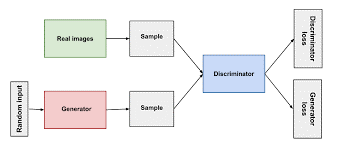
\includegraphics[width=0.6\columnwidth, ]{GAN.png}
\end{center}


\bigskip
de samenwerking word mogelijk gemaakt door het gebruik van 2 neurale netwerken die beter worden door dat ze tegenstrijdig
met elkaar werken. ze zorgen voor elkaars vooruitgang. De generator en discriminator moeten ongeveer op zelfde niveau werken als een
van de twee veel beter is dan de andere zal de gene die de fouten maakt steeds negatieve feedback
krijgen en is er een grote kans dat het model niet meer zal verbeteren (mogelijkheid tot verslechting).
\autocite{Weng2017}

\subsection{Vrianional autoencoders}
Een autoencoder pakt een afbeelding, vector, … en zal deze door een neural network laten lopen om de data
te compressen tot iets kleiner dit proces gebeurd in de encoder en stopt aan de bottle neck
(deel met de minste knopen in het neurale netwerk). Van de bottleneck willen we de data terug reprezenteren
op een hoger level (meer details krijgen in data) , dit word gedaan door de decoder. Het doel van dit
proces is om model te maken dan data kan encoden tot een kleiner level en dan terug kan decoden. Dit kan
bijvoorbeeld gebruikt worden om een afbeelding te sturen over internet met een kleinere bandbreedte en dan
op je lokaal toestel terug te decoder naar de originele afbeelding of een representatie daarvan.


\begin{center}
    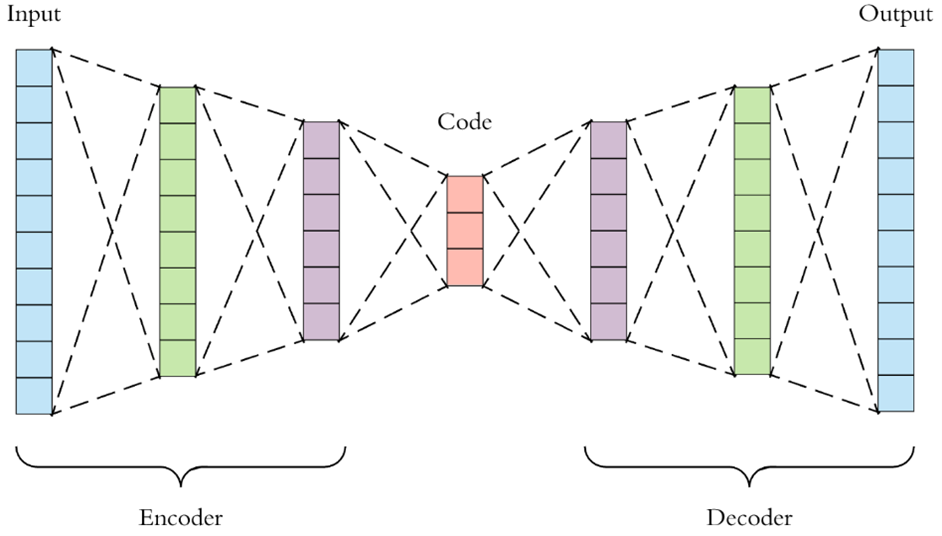
\includegraphics[width=1\columnwidth]{autoencoder.png}
\end{center}

\bigskip
We kunnen de loss functie bereken door het resultaat van de input data te vergelijken met de output data.
Met dit principe zullen we ook het neurale netwerk verbeteren bij het trainen van het model.

\bigskip
Het idee van een variational autoencoder is dat de bottleneck vector nu word opgesplitst in twee delen.
De ene representeert het gemiddelde van de distributie en de andere representeert de standaard afwijking van de distributie.
Daarmee bedoel ik dat in plaats dat we onze image hebben gelinkt aan een vector hebben we deze gekoppeld aan een distributie.

\bigskip
De data van de autoencoder is gegroepeerd via hun klasse maar de klassen zijn verspreid zijn de latend space.
Bij variational autoencoders duwen we alle data samen om de distributie te  regulariseren.
Indien we dit niet doen en we pakken een sample van de latend space dat niet in een van de klassen was
zal deze data random zijn/lijken. Bij Vrianional autoencoders  als we een sampel pakken van de lated space
dat tussen andere sampels liggen waarop we getraind hebben zal het model deze proberen combineren een nieuwe
gegenereerde waarde bekomen.
\autocite{Weng2018}

\begin{center}
    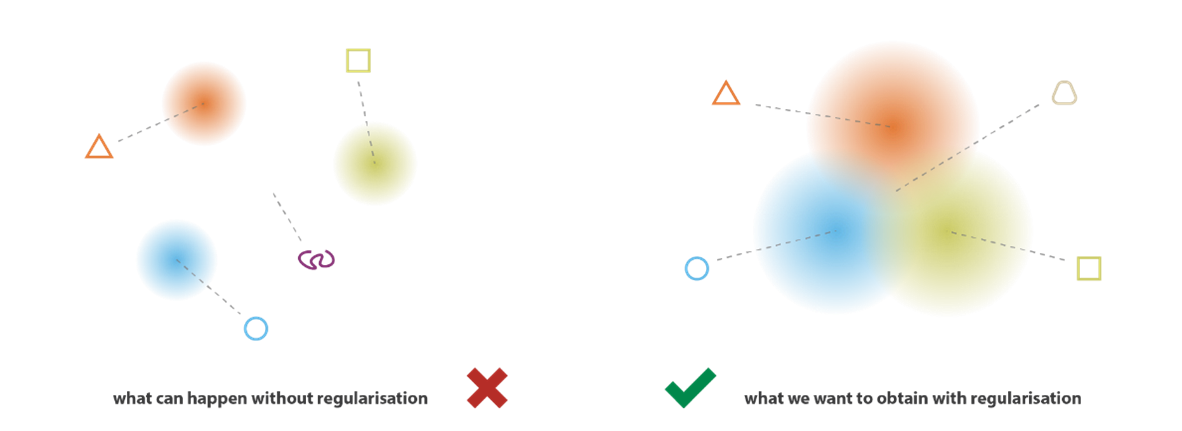
\includegraphics{VAE.png}
\end{center}

\subsection{Flow bassed models}
flow based models hebben een paar gelijkenissen met VEA doordat ze ook een afbeeling kunnen encoden naar de lated spaice
en gedecoderd terug uit de latend space. alleen noemt onze enecoder een flow en implimenteerd hij de functie f(x).
de decoder is de inverse van de functie. Dit beteken dat we alleen maar de encoder moeten trainen, de decoder zal de
invers gebruiken van de flow. Omdat we dit doen moeten de input data in de zelfde dimentie zijn als de geëncoderde data
maar wel normaal gedistributeerd. flow bassed models maken gebruik van het principe normalized flows.

\bigskip
met normalizing flows gaan we van x, een complexe distributie 
Een flow pakt x van een complex distributie en mapt deze in z als simple distributie stapsgewijs, met gebruik van een omkeerbare functie
kunnen we van z terug x zoeken.

\begin{center}
    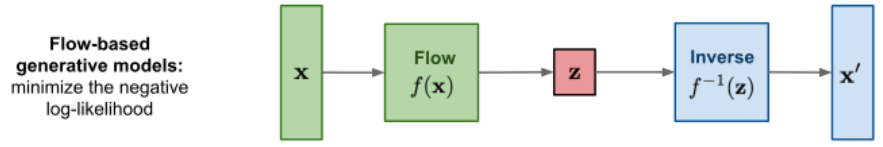
\includegraphics[width=1\columnwidth]{flow.png}
\end{center}

\subsection{Diffusion models}
Diffucion models is het nieuwste genrative model dat gebruikt word om text om te zetten naar een afbeelding.
deze modelen worden nog niet lang gebruikt maar met de grote vooruitgangen in diffusion models voor image generation
is er nu veel aandacht aan de technologie.

GLIDE gebruikt een deffucion model voor image generatie. Om een diffusie model te trainen zal je geleidelijk
aan gaussian noise (ruis) aan een afbeelding toevoegen Dit gebeurd in kleine stappen en elke stap word opgeslagen.
Dit proces stopt tot dat  de afbeelding alleen uit ruis bestaat in theorie zal dit oneindig zijn
om een prefect model te bekomen maar in praktijk doen we dit een hoog aantal keer tot de afbeelding
niet meer herkenbaar is. Hoe meer je deze stapt doet he beter de resultaten zullen zijn.

\bigskip
Na de forward noizing proces proberen we nu de noize te onderscheiden van de afbeelding door middel van 
neurale netwerken. Dit gebeurd voor elke stap die we gemaakt hebben in de forward noizing proces.
Zo hebben veel training data voor elke stap in de pipeline. Dit concept noemen we backward diffusion proces.
\autocite{Weng2021}


\begin{center}
    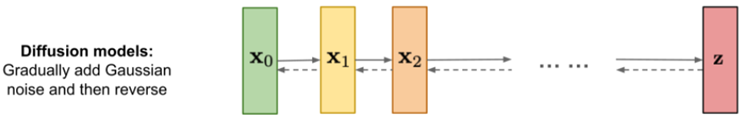
\includegraphics[width=1\columnwidth]{diffusion.png}
\end{center}

\section{GLIDE}

achter het glide model zit een neural netwerk getrained op foto's en hun beschrijving, door deep learing
kan het niet alleenn individuele objectjen begrijpen maar ook de relaties tussen de objecten.
waardoor als je een beschrijving geeft zoals: "een muis dat een huis bouwt" het ook die afbeeling kan geven.
wat zo spectaculair is aan deze technologie is dat het kan gebruiken wat het geleerd heeft van allemaal verschillende afbeeldingen 
het kan toepassen in een nieuwe te generenen afbeelding.

\subsection{Mogelijkheden van de GLIDE}
Hoewel het model een breed scala aan tekstprompts zero-shot -- Het vermogen om een taak op te lossen zonder
trainingsvoorbeelden te ontvangen (\textcite{RomeraParedes2015}) kan weergeven, kan het moeite hebben met het produceren van realistische
afbeeldingen voor complexe prompts.

\begin{center}
    \includegraphics[width=1\columnwidth]{GLIDE.png}
\end{center}

\bigskip
We kunnen niet alleen een fotos genereren maar we kunnen onderdelen aan een afbeeling toevoegen of veranderen,
dit noemen we image impainting. Dit proces heeft ons de mogelijkheid om een deel in de afbeeling te pakken
en dit te vervangen met iets anders dat de stijl van de afbeelding steeds zal volgen. GLIDE is goed model om je realisme in je
afbeeling te behouden. Natuurlijk zal het niet gewoon het te vervangen deel at random vervangen. GLIDE maakt het
mogelijk om via een textpromt het gewenste deel in de afbeeling aan de hand van de beschrijving aan te passen. 

\begin{center}
    \includegraphics[width=1\columnwidth]{GLIDE2.png}
\end{center}


\subsection{Trainen van het GLIDE model}
OpenAI heeft Het GLIDE model op 2 manieren getraind. De eerste manier dat ze probeerden was de classefier
free guidance, de ander manier maakt gebruik van het CLIP model.

\bigskip
We kunnen een model genaamed Clip als classifier te gebruik in samenwekring met GLIDE.
CLIP kan een afbeelding beoordelen aan de hand van een beschrijving over de afbeelding,
werd ook gemaakt door openAI. Met CLIP kan een computer evalueren hoe goed een tekst een afbeelding beschrijft
en zal daar een score aan geven. Het CLIP model werd ook gebruikt in samenwerking met andere modellen zoals GAN’s.
In dit geval maken we gebruik van een classefier guidance. 
\Autocite{Radford2021} 

\bigskip
het probleem met een classifier guidance is dat het een extra classifier model nodig heeft, en dat compliceerd
de training pipeline. dit model moet getraind worden op data met ruis op, dus is het niet mogelijk om het aan een standaard pretraind classifier te hangen.
We onderzoeken andere mogelijkheiden om de denoising loss fuctie bij diffusie te verminderen.
we krijgen het zelfde rezultaat of een verbetering in het
percentaal kwaliteit gemeten aan de hand van de
Inception score --"a metric for automatically evaluating the quality of image generative models" (Salimans et al., 2016)
zonder we een extra classifier nodig hebben. we noemen deze nieuwe methode classifier-free guidance.
\autocite{Ho2021}

\bigskip
"Classifier-free guidance has two appealing properties. First, it allows a single model to leverage its own
knowledge during guidance, rather than relying on the knowledge of a separate (and sometimes smaller)
classification model. Second, it simplifies guidance when conditioning on information that is difficult to
predict with a classifier (such as text).”
\textcite{Nichol2021}



\bigskip
Beide modellen zijn zeer goed voor hun doeleinde, maar we zien dat als we de Classifier-free guidance gebruiken we
beter resultaten bekomen. Dit in onder andere door dat het model meer vrijheid heeft doordat het clip model
gelimiteerd word door de imperfecties in het model.



\section{Na woordje}
In het verloop van het schrijven van deze paper heeft OpenAI nog een model uitgebracht genaamd DALL·E 2.
Net zoals GLIDE kan model ook afbeeldingen maken van een beschrijving en ze maken ook allebij gebruik van diffusion models.
waar we bij GLIDE geen clip gebruikten om een beter rezultaat te bekomen is CLIP ingebouwed in het model bij DALL·E 2.
DALL·E 2 is weer een grote grote verbetering op zijn voorgangers waaronder ook CLIP.

\begin{center}
    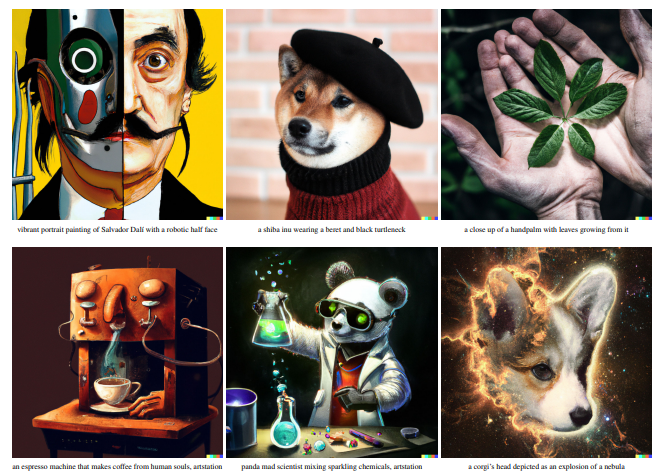
\includegraphics[width=1\columnwidth]{dall-e-2.png}
\end{center}

\bigskip
DALL·E 2 is OpenAI beste werk tot nu toe. het maakt gebruik van van technologien die we hier ook besproken hebben.

\begin{itemize}
    \item het gebruikt VAE om de beschrijving van afbeelingen te encoden.
    \item maakt gebruik van clip om afbeelingen samen mijn hun geëncode beschrijving in de latend space te compressen(iets wat GLIDE niet doet).
    \item het gebruikt een diffusion models (GLIDE was de voorganger) om de afbeeling te generenen.
\end{itemize}

\bigskip
\printbibliography
\end{document}